\chapter{Ancillary calculations}


\section{Preparatory (weather) variables}


The daily average temperature is calculated as the average of the daily minimum and the maximum
temperature. This average temperature \={T} is equal to the so called air temperature (T) used
in the model calculations. The maximum and minimum temperatures are measured daily values or
derived from other sources such as a weather forecasting model.

\begin{equation}
T ~=~{\frac{T _{\max } ~+~ T _{\min } }{2}}
\end{equation}

Where:\\[5pt]
\begin{tabularx}{\textwidth}{llXr}
	T &:& Average daily air temperature & [\textdegree C]\\
	T$_{{\rm max}}$&:  & Maximum temperature & [\textdegree C]\\
	T$_{{\rm min}}$&: &  Minimum temperature & [\textdegree C]\\
\end{tabularx}

Similarly, the daytime average temperature can be estimated as: 

\begin{equation}
% eq 5.32
\label{eq:daytimetemp}
T_{day} = {\frac{T_{\max} + T}{2}} ~~~~ where ~~~~ T = {\frac{T_{\max } + T_{\min}}{2}}
\end{equation}

The difference between maximum and minimum temperature is used to calculate the
empiric constant of the wind function in the Penman equation.

\begin{equation}
\Delta T ~= ~T _{\max } ~-~ T _{\min } 
\end{equation}

Where:\\[5pt]
\begin{tabularx}{\textwidth}{llXr}
	$\Delta$T& :& Temperature difference  &[\textdegree C]\\
	T$_{{\rm max}}$ &:& Maximum temperature &  [\textdegree C]\\
	T$_{{\rm min}}$& :& Minimum temperature  &[\textdegree C]
\end{tabularx}


As will be explained later in \S \ref{sec:penman}, the evaporative demand, EA, depends on the 
windspeed and the difference between saturated and actual vapor pressure. The windspeed
dependency is incorporated in the evaporative demand as the windspeed measured at a
height of two meters, and multiplied by an empirical coefficient (see also eq. 
\ref{eq:EvapDemand}). This
coefficient is temperature dependent and can be calculated as (Fr\`{e}re, 1979):

\begin{align}
\label{eq:BU}
BU &= 0.54 ~+ ~0.35\,{\frac{\Delta T\, - 12}{4}} & for~~~\Delta ~ T~\ge ~ 12 \degrees C \\[1em]
\nonumber
BU &= 0.54 & for~~~\Delta ~ T~<~12 \degrees C
\end{align}

Where:\\[5pt]
\begin{tabularx}{\textwidth}{llXr}
	BU & :& Empirical coefficient in the wind function &  [-]\\
	$\Delta$T& :& Temperature difference & [\textdegree C] \\
\end{tabularx}
\hspace*{6em}

The air temperature can be used to calculate the latent heat of vaporization: 

\begin{equation}
{\it \lambda} ~=~ 2.501~ -~ (2.361 \cdot 10^{-3} )\, T
\end{equation}

Where:\\[5pt]
\begin{tabularx}{\textwidth}{llXr}
	$\lambda$& :& Latent heat of vaporization & [MJ kg$^{{\rm -1}}$]\\
	T &:& Average daily temperature & [\textdegree C]\\
\end{tabularx}


As the value of the latent heat varies only slightly over normal temperature ranges a
single value for $\lambda$ may be taken. In the model for $\lambda$ a value of 2.45 MJ 
kg$^{{\rm -1}}$ is assumed (T=20 \textdegree C). The barometric pressure at sea level is 
used to calculate the psychrometric constant at sea level (Brunt, 1932).

\begin{equation}
\gamma _{o} ~=~ {{\frac{\it C _{p} \, P _{o} }{{\it  \epsilon \, \lambda } }} }\, 10 ^{-3} ~=~ 0.00163\,{\it P} _{\frac{o}{\it \lambda}} 
\end{equation}

Where:\\[5pt]
\begin{tabularx}{\textwidth}{llXr}
	$\gamma$$_{{\rm o}}$ & :& Psychrometric constant at sea level & [kPa 
	\textdegree C$^{{\rm -1}}$]\\
	C$_{{\rm p}}$ & :& Specific heat of moist air = 1.013 10$^{{\rm -3}}$ & [MJ kg$^{{\rm -1}}$ 
	\textdegree C$^{{\rm -1}}$]\\
	P$_{{\rm o}}$ & :& Atmospheric pressure at sea level & [kPa]\\
	$\epsilon$ & :& Ratio molecule weight water vapor / dry air = 0.622 & []\\
	$\lambda$ & :& Latent Heat of vaporization & [MJ kg$^{{\rm -1}}$]\\
\end{tabularx}


In the model however, a fixed value of $\gamma$$_{{\rm o}}$ = 0.67 is assumed. This 
value can be obtained by using for P the atmospheric pressure at sea level, which is 
assumed to be 101.3 kPa and $\lambda$ = 2.45 MJ kg$^{{\rm -1}}$. It should be mentioned, 
that the barometric pressure changes with altitude, so does also the psychrometer constant. 
Therefore, the two following equations are used to correct for altitude difference.

\begin{equation}
P~=~P _{o} \, e ^{{\frac{-0.034\, z}{T\, +\, 273}} }
\end{equation}

Where:\\[5pt]
\begin{tabularx}{\textwidth}{llXr}
	P &:& Atmospheric pressure at elevation z  & [kPa]\\
	P$_{{\rm o}}$ &:& Atmospheric pressure at sea level  & [kPa]\\
	T &:& Daily temperature  & [\textdegree C]\\
	z &:& Elevation  & [m]
\end{tabularx}

\begin{equation}
\label{eq:Psycho}
\gamma ~=~ \gamma _{o} \,{\frac{P}{P _{o} }}
\end{equation}

Where:\\[5pt]
\begin{tabularx}{\textwidth}{llXr}
	$\gamma$ &:& Psychrometric constant at elevation z & [kPa \textdegree C]\\
	$\gamma$$_{{\rm o}}$ &:& Psychrometric constant at sea level & [kPa \textdegree C]\\
	P &:& Atmospheric pressure at elevation z & [kPa]\\
	P$_{{\rm o}}$ &:& Atmospheric pressure at sea level & [kPa]\\
\end{tabularx}

The saturated vapor pressure is related to the mean daily air temperature and may be
approxi\-mated with the equation of Goudriaan (1977). 

\begin{equation}
\label{eq:SVP}
e_{s} ~=~ 0.610588\, \cdot \, e ^{{\frac{17.32491\, T}{T\, +\, 238.102}} }
\end{equation}

Where:\\[5pt]
\begin{tabularx}{\textwidth}{llXr}
	e$_{{\rm s}}$ &:& Saturated vapor pressure  & [kPa]\\
	T &:& Air temperature & [\textdegree C]
\end{tabularx}

From this equation the derivate, i.e. the slope of the saturated vapor pressure-temperature
curve is established.

\begin{equation}
\label{eq:SlopeSVP}
\Delta ~=~{\frac{238.102 \cdot 17.32491 \cdot e_{s} }{(T + 238.102)^{2} }}
\end{equation}

Where:\\[5pt]
\begin{tabularx}{\textwidth}{llXr}
	$\Delta$ &:& Slope of the saturation vapor pressure curve  & [kPa \textdegree C$^{{\rm -1}}$]\\
	e$_{{\rm s}}$ &:& Saturated vapor pressure &  [kPa]\\
	T &:& Air temperature & [\textdegree C]
\end{tabularx}

The measured vapor pressure is not allowed to exceed the calculated saturated vapor
pressure.

\section{Methods to estimate global radiation}

In case no observations for the incoming solar radiation are available, the formula
postulated by \AA ngstr\"{o}m (1924) can be used to estimate this parameter using sunshine
duration observations.

\begin{equation}
\label{eq:GlobRad}
S _{g,d} ~=~S _{o,d} \, (A\, +\, B\,{\frac{n}{D}} )
\end{equation}

Where:\\[5pt]
\begin{tabularx}{\textwidth}{llXr}
	S$_{{\rm g,d}}$ &:& Incoming daily global solar radiation  & [J m$^{{\rm -2}}$ d$^{{\rm -1}}$]\\
	S$_{{\rm o,d}}$ &:& Daily extra-terrestrial radiation (see eq. \ref{eq:Angot}) 
	& [J m$^{{\rm -2}}$ d$^{{\rm -1}}$]\\
	A &:& Empirical constant  & [-]\\
	B &:& Empirical constant  & [-]\\
	n &:& Bright sunshine hours per day  & [hr]\\
	D &:& Astronomical day length (see e.q. \ref{eq:irrad_diffuse})  & [hr]
\end{tabularx}

It should be mentioned that the empirical constants A and B of the \AA ngstr\"{o}m formula 
can be found with linear regression by comparing the incoming global radiation with the
relative sunshine duration n/D, taking into consideration the daily extra-terrestrial
radiation. A is the intercept and B the slope of the regression. It should also be mentioned
that the regression constants A and B have a physical meaning. A can be considered as
the fraction of extra terrestrial radiation on overcast days. The sum of A and B can be
considered as the fraction of radiation received on clear days.
For several regions in Europe the \AA ngstr\"{o}m constants have been established by Supit
(1994). Indicative values for empirical constants in the \AA ngstr\"{o}m formula are 
depicted in Table \ref{tab:angstAB}.

\begin{table}
	\centering
	\caption{Indicative values for empirical constants in the \AA ngstr\"{o}m formula in
		relation to latitude and climate used by the FAO (Fr\`{e}re \& Popov, 1979)}
	\label{tab:angstAB}
	\begin{tabular}{lcc}
		\hline
		Zone &   A &  B  \\
		\hline
		Cold and temperate zones   &  0.18 &  0.55\\
		Dry tropical zones  &   0.25  & 0.45\\
		Humid tropical zones  &   0.29 &  0.42\\
		\hline
	\end{tabular}
\end{table}

It should be clear that the constants {\bf A} and {\bf B} should be
provided by the user. As an alternative, the method developed by Supit
(1994) can be applied. This method calculates the incoming global
radiation as a function of cloud cover and sunshine duration. It can be considered as an
extension of the formula developed by Hargreaves (1985). 
Using this method, the accuracy of the results is slightly less in comparison to 
the results obtained with the \AA ngstr\"{o}m formula.

\begin{equation}
S _{g,d} ~=~ c _{a} \, S _{o,d} \, (\sqrt{(T _{\max} ~-~T _{\min} )} ~+~ 
c _{b} \sqrt{(1-{Cloud/8})} ~) ~+~c _{c} 
\end{equation}

Where:\\[5pt]
\begin{tabularx}{\textwidth}{llXr}
	S$_{{\rm g,d}}$ &:& Incoming daily global solar radiation  & [J m$^{{\rm -2}}$ d$^{{\rm -1}}$]\\
	S$_{{\rm o,d}}$ &:& Daily extra-terrestrial radiation (see eq. \ref{eq:Angot})  & 
	[J m$^{{\rm -2}}$ d$^{{\rm -1}}$]\\
	Cloud &:& Mean total cloud cover during daytime  & [octas]\\
	T$_{{\rm max}}$ &:& Maximum temperature  & [\textdegree C]\\
	T$_{{\rm min}}$ &:& Minimum temperature  & [\textdegree C]\\
	c$_{{\rm a}}$,c$_{{\rm b}}$,c$_{{\rm c}}$ &:& Empirical regression constants   & [-]
\end{tabularx}

For five regions in Europe the constants c$_{{\rm a}}$, c$_{{\rm b}}$ and c$_{{\rm c}}$ 
have been established (Supit, 1994).

Finally, in case no observations of either incoming radiation, sunshine duration and
cloudcover are available, this formula, will be used. The accuracy of this method is less
then the accuracy of the two earlier mentioned methods.

\begin{equation}
S _{g,d} ~=~ c _{d} \, S _{o,d} \, \sqrt{(T _{\max} ~-~T _{\min} )} ~+~c _{e} 
\end{equation}

Where:\\[5pt]
\begin{tabularx}{\textwidth}{llXr}
	S$_{{\rm g,d}}$ &:& Incoming daily global solar radiation  & [J m$^{{\rm -2}}$ d$^{{\rm -1}}$]\\
	S$_{{\rm o,d}}$ &:& Daily extra-terrestrial radiation (see eq. \ref{eq:Angot})  & 
	[J m$^{{\rm -2}}$ d$^{{\rm -1}}$]\\
	T$_{{\rm max}}$ &:& Maximum temperature  & [\textdegree C]\\
	T$_{{\rm min}}$ &:& Minimum temperature  & [\textdegree C]\\
	c$_{{\rm d}}$,c$_{{\rm e}}$  &:& Empirical regression constants  & [-]\\
\end{tabularx}

For six regions in Europe the constants c$_{{\rm d}}$ and c$_{{\rm e}}$ have been 
established (Supit, 1994). In section \ref{sec:daylength} it is explained how the 
daily extra-terrestrial radiation, S$_{{\rm o,d}}$, can be calculated.

\section{Reference evapotranspiration}

Transpiration is the loss of water from the plants and evaporation is the
loss of water from the soil or from a free-water surface. Evapotranspiration covers both
transpiration and evaporation.
The principal driving force for evaporation is the gradient of vapour pressure between the
evaporating surface and the surrounding air. The vapour pressure at the evaporating
surface is equal to the saturated vapour pressure at the prevailing temperature of that
surface. The vapour pressure of the air is a function of the ambient temperature and its
relative humidity. The rate of evaporation depends on the diffusion resistance between the
evaporating surface and the air.
The magnitude of the resistance is strongly related to wind speed. The two environ\-mental
variables, air humidity and wind speed combined determine the 'evaporative demand' of
the air.

The problem in the approach above is that the temperature of the evaporating surface is
usually not known from standard meteorological observations. Evaporation  of 1 mm
layer of water requires 2.45 MJ m$^{{\rm -2}}$ of energy and can therefore be described through
quantification of an energy balance. The energy dissipation, required for evaporation,
leads to cooling of the evaporating surface which reduces the vapour gradient. Hence, a
driving force is required to maintain the corresponding surface temperature, and thus,
maintain the vapour pres\-sure gradient. The energy for this driving force is supplied by the
net solar radiation received by the canopy and or soil.
Net radiation is the balance between incoming (short-wave) radiation from the sun and
radiation losses due to reflection and outgoing (long-wave) radiation. 

Heat supplied by
moving air is another source of energy, but this is usually negligible, except in situations
where the vegetation is surrounded by extensive bare areas (oasis). Only 5-8\% of
incoming radiation is dissipated in photosynthesis, which is, therefore, disregarded here.
Respiration yields an insignificant amount of energy. To simplify the treatment of
evapotranspiration, it is considered to be governed by two factors: radiation and evaporative demand.

Penman (1948) was the first to describe evapotranspiration in physical mathematical
terms. He calculated evaporation from free-water surfaces, wet bare soil and low grass
swards for 10-day periods. The original Penman reference evapotranspiration has now been 
superseded by the 
Penman-Monteith reference evapotranspiration. The latter has a better physical basis and
is standardized and promoted by the Food and Agriculture Organization. WOFOST uses the
Penman-Monteith equation to compute the crop reference evapotranspiration but still applies
the older Penman approach as reference evapotranspiration for open water and bare soil.
Moreover, the option to use the older Penman approach as reference evapotranspiration is still
available in order to compare with historical studies.

The value calculated according to the Penmn and Penman-Monteith equations is the potential 
evapotranspiration $ET0$, i.e. without limitations with respect to the supply of liquid water to the
evaporating surface. This $ET0$ value is often used as a reference value, to
which actual crop water demand is related. To translate $ET0$ into crop water require\-ments,
so called crop factors can be used (e.g. Doorenbos \& Pruitt, 1977; Feddes {\it et al.},
1978). See also \S \ref{sec:evapotranspiration}.

Note that the equations used to compute $ET0$ provide the value in mm/day while internally
this is converted into cm/day.

\subsection{Terms in the Penman formula}
\label{sec:penman}

The Penman formula (equation \ref{eq:ET0}) consists of two segments. The first part, the radiative
term, calculates the net absorbed radiation. The second part, the aerodynamic term,
calculates the evapora\-tive demand of the atmo\-sphere (Choisnel {\it et al}., 1992; Fr\`{e}re and
Popov, 1979; Penman, 1956, 1948). The resulting equations are used to calculate the
potential evapora\-tion rates from a water surface, from bare soil surfaces and the potential
evapotranspira\-tion rate from a crop canopy.

\begin{equation}
\label{eq:ET0}
ET0 ~=~ W ~R _{na} ~+~(1\, -\, W) ~E _{a} 
\end{equation}

Where:\\[5pt]
\begin{tabularx}{\textwidth}{llXr}
	ET0&:& Evapo(transpi)ration & [mm d$^{{\rm -1}}$] \\
	W&:& Temperature related weighing factor &  [-] \\
	R$_{{\rm na}}$&: & Net absorbed radiation in equivalent evaporation & [mm d$^{{\rm -1}}$] \\
	EA&: &  Evaporative demand in equivalent evaporation & [mm d$^{{\rm -1}}$] \\
\end{tabularx}

The temperature related weighing factor W in equation \ref{eq:ET0} is defined as 
(Fr\`{e}re and Popov, 1979; Penman, 1948, 1956).

\begin{equation}
W ~=~{\frac{\Delta}{(\Delta ~+~ \gamma )}} 
\end{equation}

Where:\\[5pt]
\begin{tabularx}{\textwidth}{llXr}
	$\Delta$ &:& Slope of the saturation vapor pressure curve (see eq. \ref{eq:SlopeSVP})  & [kPa \textdegree C$^{{\rm -1}}$]\\
	$\gamma$ &:& Psychrometric constant (see eq. \ref{eq:Psycho})  & [kPa \degrees C$^{{\rm -1}}$]
\end{tabularx}

To calculate net outgoing long wave radiation Penman (1956) used an equation which is
derived from the formula postulated by Brunt (1932). The net outgoing long wave
radiation increases with increasing values for the mean air temperature and the relative
sunshine duration and decreases with increasing vapor pressure.

\begin{equation}
R _{nl} \uparrow  ~=~ \sigma \,\, (T+273) ^{4} \,\, (0.56\,\, -\,\, 0.079\, \sqrt{e _{a} } )\,\, (0.1\,\, +\,\, 0.9\,\,{\frac{n}{D}} )
\end{equation}


Where:\\[5pt]
\begin{tabularx}{\textwidth}{llXr}
	R$_{{\rm nl}}$$\uparrow$ &:& Net outgoing long-wave radiation & [J m$^{{\rm -2}}$ d$^{{\rm -1}}$]\\
	$\sigma$ &:& Stefan Boltzm\-ann constant = 4.90 x 10$^{{\rm -9}}$ & [J m$^{{\rm -2}}$ K$^{{\rm -4}}$ s$^{{\rm -1}}$]\\
	T &:& Air temperature & [\textdegree C]\\
	e$_{{\rm a}}$ &:& Actual vapor pressure & [kPa]\\
	n/D &:& Relative sunshine duration & [-]\\
\end{tabularx}

The relative sunshine duration, n/D, is established in the model using:

\begin{equation}
{\frac{n}{D}} ~=~{\frac{T_{atm} ~-~A}{B}}
\end{equation}

Where:\\[5pt]
\begin{tabularx}{\textwidth}{llXr}
	n/D &:& Relative sunshine duration  & [-]\\
	T$_{{\rm atm}}$ &:& Atmospheric transmission (see eq. \ref{eq:Tatm})  & [-]\\
	A &:& Empirical constant in the \AA ngstr\"{o}m equation  & [-]\\
	B &:& Empirical constant in the \AA ngstr\"{o}m equation  & [-]\\
\end{tabularx}


The calculation of the atmospheric transmission, T$_{{\rm atm}}$, will be explained in 
\S \ref{sec:daylength}.

Part of the actual received radiation is reflected by the surface. The fraction reflected
(albedo) is different for a water surface, a soil surface and a crop canopy. The absorbed
fraction of radiation actually received minus the net outgoing radiation equals the net
absorbed radiation, which is divided by the latent heat of vaporization of water to express
the amount of radiation in depth of evaporative water layer (mm d$^{{\rm -1}}$).

\begin{equation}
\label{eq:AbsGlobRad}
R _{na} ~=~{\frac{(1\, -\, \alpha )\,\, R _{av} \, -\, R _{nl} \uparrow  }{\lambda}}
\end{equation}


Where:\\[5pt]
\begin{tabularx}{\textwidth}{llXr}
	R$_{{\rm na}}$ &:& Net absorbed radiation  & [mm d$^{{\rm -1}}$]\\
	$\alpha$ &:& Albedo or reflection coefficient of regarded surface  & [-]\\
	R$_{{\rm av}}$ &:& Average radiation  & [J m$^{{\rm -2}}$ d$^{{\rm -1}}$]\\
	R$_{{\rm nl}}$$\uparrow$ &:& Net outgoing long-wave radiation  & [J m$^{{\rm -2}}$ d$^{{\rm -1}}$]\\
	$\lambda$ &:& Latent heat  & [J kg$^{{\rm -1}}$]\\
\end{tabularx}


The soil's albedo depends on the surface color and on the moisture content. Albedo
values for dry soil vary from 0.14 (clay) to 0.37 (dune sand). Ten Berge (1986) described
the depen\-dence of the albedo value on soil moisture in relation to the average water
content of the top soil layer. See Table \ref{tab:AlbedoSoils}. 
In WOFOST 7.2 the following values for the albedo are assumed: for bare soil
0.15, for a canopy  0.25 and for a water surface a value of 0.05.

\begin{table}
	\centering
	\caption{Albedo values for wet and dry soils (ten Berge, 1986)}
	\label{tab:AlbedoSoils}
	\begin{tabular}{lcc}
		\hline
		soil type & wet & dry\\
		\hline
		Dune sand  &   0.24 &  0.37 \\
		Sandy loam &    0.10-0.19 &  0.17-0.23\\
		Clay loam &    0.10-0.14 &  0.20-0.23\\
		Clay &    0.08 &  0.14\\
		\hline
	\end{tabular}
\end{table}

The evaporative demand of the atmosphere depends on the difference between saturated
and actual vapor pressure and on the wind function. For crop canopies the evaporative
demand is somewhat higher than for soil or water surfaces due to a higher surface
roughness. This is reflected in a higher value for {\it factor} in the wind function.

\begin{equation}
\label{eq:EvapDemand}
EA~=~0.26\, (e _{s} \, -\, e _{a} )\,\, (factor\, +\, BU\, u(2))
\end{equation}

Where:\\[5pt]
\begin{tabularx}{\textwidth}{llXr}
	EA &:& Evaporative demand  & [mm d$^{{\rm -1}}$]\\
	e$_{{\rm s}}$ &:& Saturated vapor pressure (see eq. \ref{eq:SVP})  & [kPa]\\
	e$_{{\rm a}}$ &:& Actual vapor pressure  & [kPa]\\
	{\it factor} &:& Empirical constant  & [-]\\
	BU &:& Coefficient in wind function (see eq. \ref{eq:BU})  & [-]\\
	u(2) &:& Mean windspeed at 2 m height  & [m s$^{{\rm -1}}$]\\
\end{tabularx}

The following values for {\it factor} are assumed (Fr\`{e}re, 1979). For crop canopies {\it factor} =
1.0 and for a free water a surface {\it factor} = 0.5.

Substituting equations \ref{eq:EvapDemand} and \ref{eq:AbsGlobRad} in equation \ref{eq:ET0} yields

\begin{equation}
\label{eq:Penman}
ET0 ~=~{\frac{(\Delta R _{na~} +~\gamma EA)}{\Delta ~+~\gamma }}
\end{equation}

Where:\\[5pt]
\begin{tabularx}{\textwidth}{llXr}
	ET0 &:& Evapo(transpiration)  & [mm d$^{{\rm -1}}$]\\
	R$_{{\rm na}}$ &:& Net absorbed radiation  & [mm d$^{{\rm -1}}$]\\
	EA &:& Evaporative demand  & [mm d$^{{\rm -1}}$]\\
	$\Delta$ &:& Slope of the saturation vapor pressure curve   & [kPa \degrees C$^{{\rm -1}}$]\\
	$\gamma$ &:& Psychrometric constant  & [kPa \degrees C$^{{\rm -1}}$]
\end{tabularx}

With the equations \ref{eq:AbsGlobRad}, \ref{eq:EvapDemand}, \ref{eq:Penman} and the different values for factor and albedo, the evapo(transpi)ration from a wet bare soil surface E0$_{{\rm s}}$, a water surface, E0$_{{\rm w}}$, and a crop canopy, ET0, can be easily calculated.


\subsection{Terms in the Penman-Monteith formula}

The Penman-Monteith equation implemented in WOFOST closely follows the algorithm laid down in 
FAO Irrigation and drainage paper 56 ("Crop evapotranspiration - Guidelines for computing crop 
water requirements") by Allen et al. (1998) which is available online \footnote{http://www.fao.org/3/X0490E/x0490e00.htm}
and will not be repeated here.

Standard values for the reference canopy reflection and canopy resistance of 0.23 and 70 $s m^{-1}$ are used and
the soil heat flux is explicitly set to zero. Moreover, some of the terms in the FAO PM equation have been
rearranged for clarity. For example the magic number "0.408" in the FAO equation can be more easily 
understood as one divided by the latent heat for vaporisation.


\section{Day length and solar elevation}
\label{sec:daylength}

The ASTRO module calculates day length, some intermediate variables for the calculation
of the solar elevation, the integral of the solar elevation over a day and the fraction of
diffuse radiation.

Day length is a function of the angle of the sun above the horizon (solar elevation). Solar
elevation is the angle between the sun rays and the earth's surface. Solar elevation is
determined by latitude, the day and the hour on a certain day.
The dependency on the hour of a certain day is simple to explain. The sun rises and the
sun sets every day. Just before sun rise and just after sun set the solar elevation is zero. 
At the equator on days that the sun is in zenith (the point in the sky directly overhead) at 
12 o'clock solar time it holds that:

\begin{equation}
\sin \beta = \cos (15(t _{h} -12))
\end{equation}

Where:\\[5pt]
\begin{tabularx}{\textwidth}{llXr}
	$\beta$ &:& Solar elevation  & [degrees]\\
	t$_{{\rm h}}$ &:& Hour of the day  & [h]\\
\end{tabularx}

The angle of the sun changes during the day because the earth rotates once around its axis
every 24 hours at a speed of 15\degrees per hour (= 360/24).  

To explain the dependency of solar elevation on latitude and day number first the situation
is regarded when the sun is in zenith. This is at 12 o'clock solar time (not to be mixed up
with noon). The solar declination, the place were the sun is in zenith at 12 o'clock solar
time, changes every day. On the 21$^{\rm st}$ of June the sun stands perpen\-dicular above 
the northern tropic of Cancer (+23.45\degrees N) and on the 22$^{\rm nd}$ of December the 
stands perpendicular above the tropic of Capricorn (-23.45\degrees S). In figure 
\ref{fig:solardecl} the situation is depicted for 22$^{\rm nd}$ of December when the sun 
reaches its highest point at the tropic of Capricorn at the southern hemisphere. On the 
northern hemisphere this results in the shortest day of the year.

\begin{figure}[p]
	\centering
	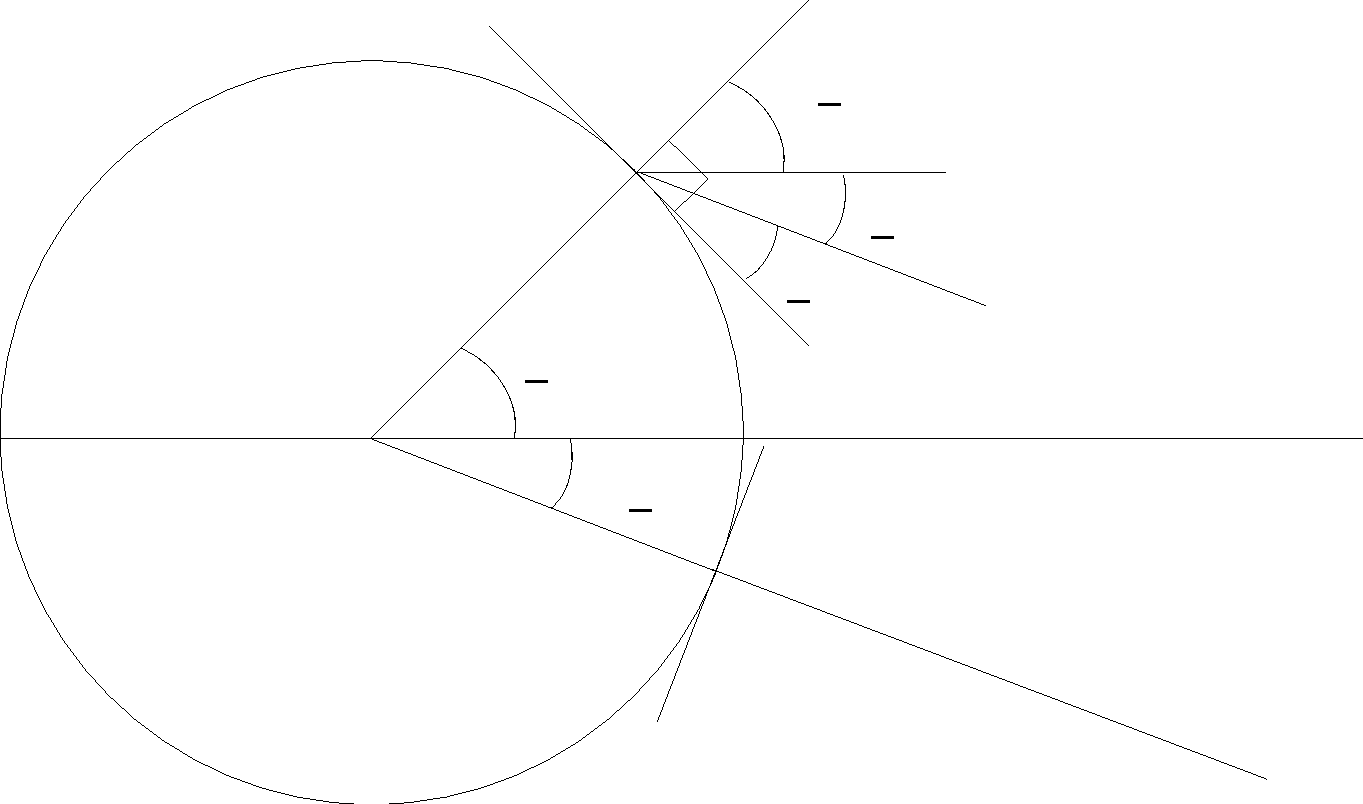
\includegraphics[width=93mm]{\FigDir/AARDE3.pdf}
	\caption{Solar declination}
	\label{fig:solardecl}
	%\begin{forcewidth}{9.33cm}
	% \begin{center}\InputPS{\FigDir/AARDE3.eps} \end{center}
	%\end{forcewidth}
\end{figure}

The solar declination during the year can be approached by a cosine function. (Note a shift of ten days).
The distance of the sun to the earth is considered to be infinite, therefore declination 
can be considered equal for all places on earth.

\begin{equation}
\delta ~=~ -23.45 \cos ( 2 \pi {\frac{t _{d} + 10}{365}} )
\end{equation}

Where:\\[5pt]
\begin{tabularx}{\textwidth}{llXr}
	$\delta$ &:& Solar declination   & [de\-grees]\\
	t$_{{\rm d}}$ &:& Number of the day since 1 January   & [-]\\
\end{tabularx}

The orbit of the earth around the sun is a
non concentric ellipse (see figure \ref{fig:orbit}), therefore the solar radiation received 
at the top of the atmosphere during the year is not constant. At the first of January the 
earth is closest to the sun, radiation at the top of the atmosphere will then be higher as 
during other days.

\begin{figure}p]
	\centering
	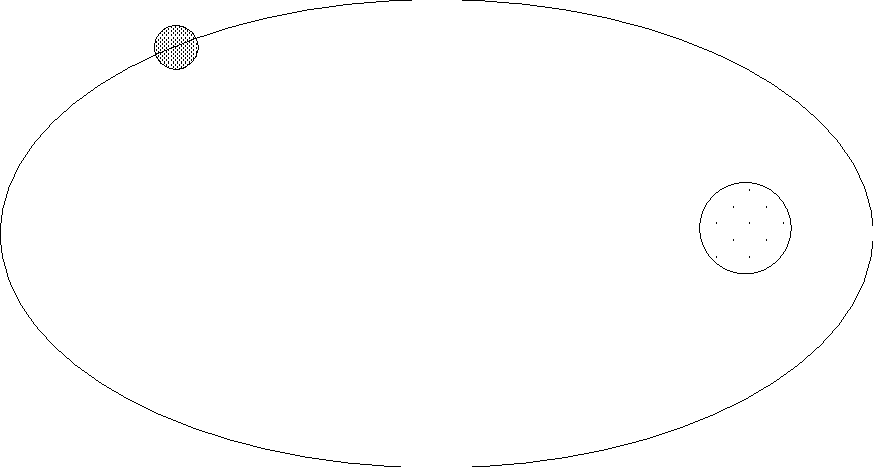
\includegraphics[width=80mm]{\FigDir/ELIPS.pdf}
	\caption{Orbit of the earth around the sun}
	\label{fig:orbit}
	%\begin{forcewidth}{7.77cm}
	%% \begin{center}\InputPS{\FigDir/ELIPS.eps} \end{center}
	%\end{forcewidth}
\end{figure}

The average solar radiation at the top of the atmosphere is estimated at 1370 W m$^{\rm -2}$. A daily solar radiation constant can than be calculated as a cosine times the average solar radiation at the top of the atmosphere multiplied by correction factor to correct for the elliptical orbit of the earth around the sun. This correction factor is estimated to be 0.033.

\begin{equation}
\label{eq:SolarConst}
S _{c,d} = S _{c} (1+0.033 \cos (2 \pi {\frac{t _{d} }{365}} ))
\end{equation}

Where:\\[5pt]
\begin{tabularx}{\textwidth}{llXr}
	S$_{{\rm c,d}}$ &:& Solar constant at the top of the atmosphere for a certain day  & [J m$^{{\rm -2}}$ s$^{{\rm -1}}$]\\
	S$_{{\rm c}}$ &:& Average solar radiation at the top of atmosphere (1370 J m$^{{\rm -2}}$ s$^{{\rm -1}}$; I.E.A., 1978) & [J m$^{{\rm -2}}$ s$^{{\rm -1}}$]\\
	t$_{{\rm d}}$ &:& Number of day since 1 January  & [-]\\
\end{tabularx}

Note that during the winter in Europe the solar radiation at the top of the atmo\-sphere is at 
its maximum! The height of the sun at any moment throughout the day and at any place and date can be
calculated using:

\begin{equation}
\label{eq:SolarElevation}
\sin \beta = \sin \lambda \sin \delta + \cos \lambda \cos \delta \cos (2 \pi {\frac{(t _{h} +12)}{24}} )
\end{equation}

Where:\\[5pt]
\begin{tabularx}{\textwidth}{llXr}
	$\beta$ &:& Solar elevation  & [degrees]\\
	$\lambda$ &:& Latitude  & [degrees]\\
	$\delta$ &:& Solar declination  & [degrees]\\
	t$_{{\rm h}}$ &:& Hour of the day (solar time)  & [h]\\
\end{tabularx}

To compute day length for photoperiod-sensitive species, it must be realized that, even
when the sun is still below the horizon the light level is high enough to trigger the
photoperiodicity mechan\-ism. Photoperiodic day length is 0.5 h longer than the 
astronomi\-cal day length at the equator and about 0.8 h in temperate zones, depending 
on the date of the year. The light level to which photoperiodism is sensitive is quite low and not well
quantified. Vergara \& Chang (1985) determined it to be 1.5-15 mW m$^{{\rm -2}}$ for 
rice crops; Salisbury (1981) determined the level to be higher. As a compromise a value of 50 mW
m$^{{\rm -2}}$ is used in the model, which corresponds with a sun angle of -4 degrees. The
photosynthetic active period and the astro\-nomical day length can be calculated as:

\begin{equation}
% eq 4.25
\label{eq:AstroDaylength}
D ~=~ 12~+~{\frac{24}{180}} \, \arcsin \, (\,{\frac{-\sin {\frac{p}{180}} + sinLD}{cosLD}} )
\end{equation}

Where:\\[5pt]
\begin{tabularx}{\textwidth}{llXr}
	D &:& Day length  & [h]\\
	sinLD &:& Seasonal offset of sine of solar height = sin$\delta$sin$\lambda$  & [-]\\
	cosLD &:& Amplitude of sine of solar height = cos$\delta$cos$\lambda$  & [-]\\
	p &:& correction constant  & [degrees]\\
\end{tabularx}

The correction constant for the photosynthetic day length is -4 degrees. For the astronomical 
day length the correction constant is -0.833 degrees (i.e. solar height for which
the upper edge of the solar disk appears on the horizon). However, in the model for the
calculation of the astronomical day length, a correction constant of 0 degrees is used. 

For locations below -66.5 and above 66.5 degrees of latitude, situations of no daylight (polar night) 
and 24h day light (e.g. polar day) occur. In such cases the calculated daylenght will be set
to zero daylength (polar night) or 24 hour day length (polar day). 

The integral of the solar height over the day can be obtained as twice the integral from
sunrise ($\beta$=0\degrees ) to 12 o'clock solar time ($\beta$ = 90\degrees  + $\delta$ - $\lambda$):

\begin{equation}
\label{eq:IntgrlSolarHeigh}
\int \sin \beta dt _{h} ~=~ 3600( D \sin \lambda \sin \delta +{\frac{24}{\pi }} \cos \lambda \cos \delta \sqrt{1-\tan^{2} \lambda \tan^{2} \delta } )
\end{equation}

Where:\\[5pt]
\begin{tabularx}{\textwidth}{llXr}
	$\int$sin$\beta$  &:& Integral solar height & [s]\\
	D  &:& Day length & [h]\\
	$\beta$  &:& Solar elevation & [degrees]\\
	t$_{{\rm h}}$  &:& Hour of the day & [h]\\
\end{tabularx}

Multiplication of equation \ref{eq:SolarConst} with \ref{eq:IntgrlSolarHeigh} yields the 
daily extra-terrestrial radiation which is also known as the Angot radiation. Note that 
the dimension of the daily extra-terrestrial is radiation J m$^{{\rm -2}}$ d$^{{\rm -1}}$.

\begin{equation}
% eq 4.27
\label{eq:Angot}
S_{o,d} = S _{c,d} ~ \int \sin \beta dt _{h} 
\end{equation}

Where:\\[5pt]
\begin{tabularx}{\textwidth}{llXr}
	S$_{{\rm o,d}}$ &:& Daily extra-terrestrial radiation  & [J m$^{{\rm -2}}$ d$^{{\rm -1}}$]\\
	S$_{{\rm c,d}}$ &:& Solar constant at the top of the atmosphere 
	for a certain day (see eq. \ref{eq:SolarConst})  & [J m$^{{\rm -2}}$ s$^{{\rm -1}}$]\\
	t$_{{\rm d}}$ &:& Number of day since 1 January  & [-]\\
\end{tabularx}

In the model the integral of the effective solar height, a modification of equation \ref{eq:Angot} is
also calculated. This modified integral takes the effect of the daily course in atmospheric
transmis\-sion into account. Transmission is lower near the margins of the day because of
haze in the morning and clouds in the afternoon. Besides that, path length of solar
radiation in the atmosphere is longer (Spitters {\it et al}., 1986). This modified integral 
can be calculated as:

\begin{align}
% eq 4.28
\label{eq:IntSolarHeight}
\int \sin \beta_{m} &= \int \sin \beta (1+csin \beta ) dt_{h}  \\
&= 3600 \cdot \left \{
\begin{tabular}{c}
$D ( \sin \lambda \sin \delta + 0.4 
(( \sin \lambda \sin \delta )^{2} + 0.5( 
\cos \lambda \cos \delta ) ^{2} )) ~ + \nonumber$ \\[1em]
${\frac{12}{\pi}} \cos \lambda \cos 
\delta (2+3 \cdot 0.4 \sin \lambda \sin \delta ) 
\sqrt{1-\tan^{2} \lambda \tan^{2} \delta } \nonumber$
\end{tabular}
\right \}
\end{align}

Where:\\[5pt]
\begin{tabularx}{\textwidth}{llXr}
	$\int \sin \beta_{m}$  &:& Integral of effective solar height   & [s]\\
	D  &:& Day length       & [h]\\
	c  &:& Coefficient of regression on transmission on solar angle = 0.4  & [-]\\
	$\beta$  &:& Solar elevation   & [degrees]\\
	$\lambda$  &:& Latitude   & [degrees]\\
	$\delta$  &:& Solar declination   & [degrees]\\
	t$_{{\rm h}}$  &:& Hour of the day  f & [h]\\
\end{tabularx}

A distinction is made between diffuse sky light, with incidence under various angles and
direct sunlight with an angle of incidence equal to the solar declination. It is important 
to distin\-guish these fluxes because of the large difference in illumination intensity 
between shaded leaves and sunlit leaves and therefore the difference in the CO$_{{\rm 2}}$ 
assimila\-tion light response of single leaves, which is non-linear. Shaded leaves receive 
only diffuse radiation. Sunlit leaves receive both direct and diffuse radiation. The 
diffuse flux is the result of the scattering of sun rays by clouds, aerosols and gases in 
the atmo\-sphere. The propor\-tion of diffuse light in the total incident light flux depends 
on the status of the atmosphere, i.e. cloudi\-ness, concentra\-tion of aerosols. This 
fraction is calculated from the atmospheric transmis\-sion using an empirical function. 
This relationship is based on data from different meteorologi\-cal stations from a wide 
range of latitudes and longitudes (Spitters {\it et al}., 1986). 

The atmospheric transmission is the ratio between actual radiation and the quantity that
would have reached the earth's surface in the absence of an atmosphere (i.e. Angot
radiation). This ratio can be calculated as:

\begin{equation}
\label{eq:Tatm}
T _{atm} ~=~ s _{\frac{g,d}{S _{c,d} \int \sin \beta }}
\end{equation}

Where:\\[5pt]
\begin{tabularx}{\textwidth}{llXr}
	T$_{{\rm atm}}$ &:& Atmospheric transmission  & [-]\\
	S$_{{\rm g,d}}$ &:& Daily global radiation  & [J m$^{{\rm -2}}$ d$^{{\rm -1}}$]\\
	S$_{{\rm c,d}}$ &:& Solar constant at the top of the atmosphere for a certain day 
	(see eq. \ref{eq:SolarConst} and \ref{eq:Angot})  & [J m$^{{\rm -2}}$ s$^{{\rm -1}}$]\\
	$\int \sin \beta$  &:& Integral of solar height   & [s]\\
\end{tabularx}

Relationships between the share of the diffuse flux in the global irradiance 
(S$_{{\rm df}}$/S$_{{\rm g}}$) and the atmospheric transmission 
(S$_{{\rm g}}$/S$_{{\rm o}}$) are found in several research reports concerning the use
of solar energy in solar collectors. The relation is characterized by an approximately
linear trend for transmissions ranging between 0.35 and 0.75. At low transmissions,
nearly all of the incoming radiation is diffuse so that the curve bends off.
There is some variation among published relations, arising from differences in atmospheric 
conditions, especially relative sunshine duration, water content of the atmosphere,
and cloud type, but also lack of fit of the presented regression equation from the data and
differences in the method of measuring the diffuse radiation.

The relation used in WOFOST Version 7.2 has been derived by de Jong (1980) and has
been recommended by Spitters {\it et al}. (1986).

\begin{align}
% eq 4.30
\label{eq:irrad_diffuse}
{\frac{S _{df,d} }{S _{g, d} }} &= 1 & 
for ~~ {\frac{S _{g,d} }{S _{o,d} }} \le 0.07 \nonumber \\
{\frac{S _{df,d} }{S _{g,d} }} &= 1-2.3({\frac{S _{g,d} }{S _{o,d} }} -0.07) ^{2} & 
for ~~ 0.07 < {\frac{S _{g,d} }{S _{o,d} }} \le 0.35  \nonumber \\
{\frac{S _{df,d} }{S _{g,d} }} &= 1.33-1.46{\frac{S _{g,d} }{S _{o,d} }} &
for ~~ 0.35 < {\frac{S _{g,d} }{S _{o,d} }} \le 0.75 \nonumber \\
{\frac{S _{df,d} }{S _{g,d} }} &= 0.23 &
for ~~ {\frac{S _{g,d} }{S _{o,d} }} > 0.75 \nonumber \\
\end{align}

Where:\\[5pt]
\begin{tabularx}{\textwidth}{llXr}
	S$_{{\rm df,d}}$ &:& Daily diffuse radiation  & [J m$^{{\rm -2}}$ d$^{{\rm -1}}$]\\
	S$_{{\rm g,d}}$ &:& Daily global radiation  & [J m$^{{\rm -2}}$ d$^{{\rm -1}}$]\\
	S$_{{\rm o,d}}$ &:& Daily extra-terrestrial radiation (see eq. \ref{eq:Angot})  & 
	[J m$^{{\rm -2}}$ d$^{{\rm -1}}$]\\
\end{tabularx}

The relationships are remarkably constant over climates and latitudes so that the presented
equations will be valid for a wide range of conditions (Spitters {\it et al}., 1986).

Measured or estimated daily total solar irradiation (wavelength 300-3000 nm) is input for
the model. Only half of this incoming radiation is photosynthetical active (PAR,
Photosynthetically active radiation, wavelength 400 - 700 nm). The photosynthetically active
diffuse radiation, perpendicular to the direction of the solar rays can be calculated as:

\begin{equation}
% eq 4.31
\label{eq:PAR}
D _{p} ~=~ S _{\frac{df,d}{S _{g,d} }} ~~ T _{atm} ~0.5S _{c,d} 
\end{equation}


Where:\\[5pt]
\begin{tabularx}{\textwidth}{llXr}
	D$_{{\rm p}}$ &:& Diffuse irradiation perpendicular to the direction of light  & 
	[J m$^{{\rm -2}}$ s$^{{\rm -1}}$]\\
	T$_{{\rm atm}}$ &:& Atmospheric transmission (see eq. \ref{eq:Tatm})  & [-]\\
	S$_{{\rm c,d}}$ &:& Solar constant at the top of the atmosphere for a certain day  & 
	[J m$^{{\rm -2}}$ s$^{{\rm -1}}$]\\
	S$_{{\rm g,d}}$ &:& Daily global radiation  & [J m$^{{\rm -2}}$ d$^{{\rm -1}}$]\\
	S$_{{\rm df,d}}$ &:& Daily diffuse radiation (see eq. \ref{eq:irrad_diffuse})  & 
	[J m$^{{\rm -2}}$ d$^{{\rm -1}}$]\\
\end{tabularx}


